V této kapitole jsou popsány metody použité v bakalářské práci. V podkapitole
\ref{section:measurement} je rozebrán postup měření EKG záznamů a použité
zařízení. V kapitole \ref{section:study} je charakterizována kontrolní skupina
probandů a sledované veličiny. V kapitolách \ref{section:offline_processing} a
\ref{section:online_processing} je řešena metodologie online a offline
zpracování a hodnocení EKG signálu. Kapitola \ref{section:statistical_methods}
pojednává o statistickém zpracování výsledků.

%//TODO: Kdo zajistil holter
\subsection{Měření EKG signálů}
\label{section:measurement}
Pro účely zpracování a analýzy EKG signálu, které jsou náplní této bakalářské
práce, byly naměřeny krátkodobé záznamy srdeční aktivity na 5 probandech. Postup
měření je specifikován v kapitole \ref{section:measurement_methodology}. Měřící
zařízení je blíže popsáno v následující kapitole.

\subsubsection{Měřící zařízení}
\label{section:measurement_device}
Zařízení použité k měření srdeční aktivity byl Holterův monitor
(\ref{fig:device}), zajištěný vědeckým týmem Biomechaniky a asistivních
technologií. Skládá se ze dvou komponent --- samotné zařízení a 3-svodový EKG
kabel s 3.5~\si\mm~jack konektorem. Vzorkovací frekvence zařízení je 500 \si\Hz.

Přenos dat ze zařízení probíhá bezdrátově na lokální sítí (WLAN), ke které je
třeba zařízení připojit pomocí volně dostupné mobilní aplikace \textit{ESPTouch:
    SmartConfig} podle postupu níže. \textit{ESP-TOUCH} je protokol, umožňující
vestavěným systémům (embedded systémy) jednoduché připojení k Wi-Fi sítím pomocí
chytrých mobilních zařízení \cite{esptouch}. K záznamu dat byla použita
aplikace, naprogramovaná v rámci této práce, jménem \textit{BBMP (Better bpm)},
která se zařízením komunikuje přes protokol \textit{Modbus} \cite{modbus}.
Aplikace \textit{BBPM} je blíže popsaná v kapitole
\ref{section:offline_processing}.

\begin{figure}[H]
    \begin{center}
        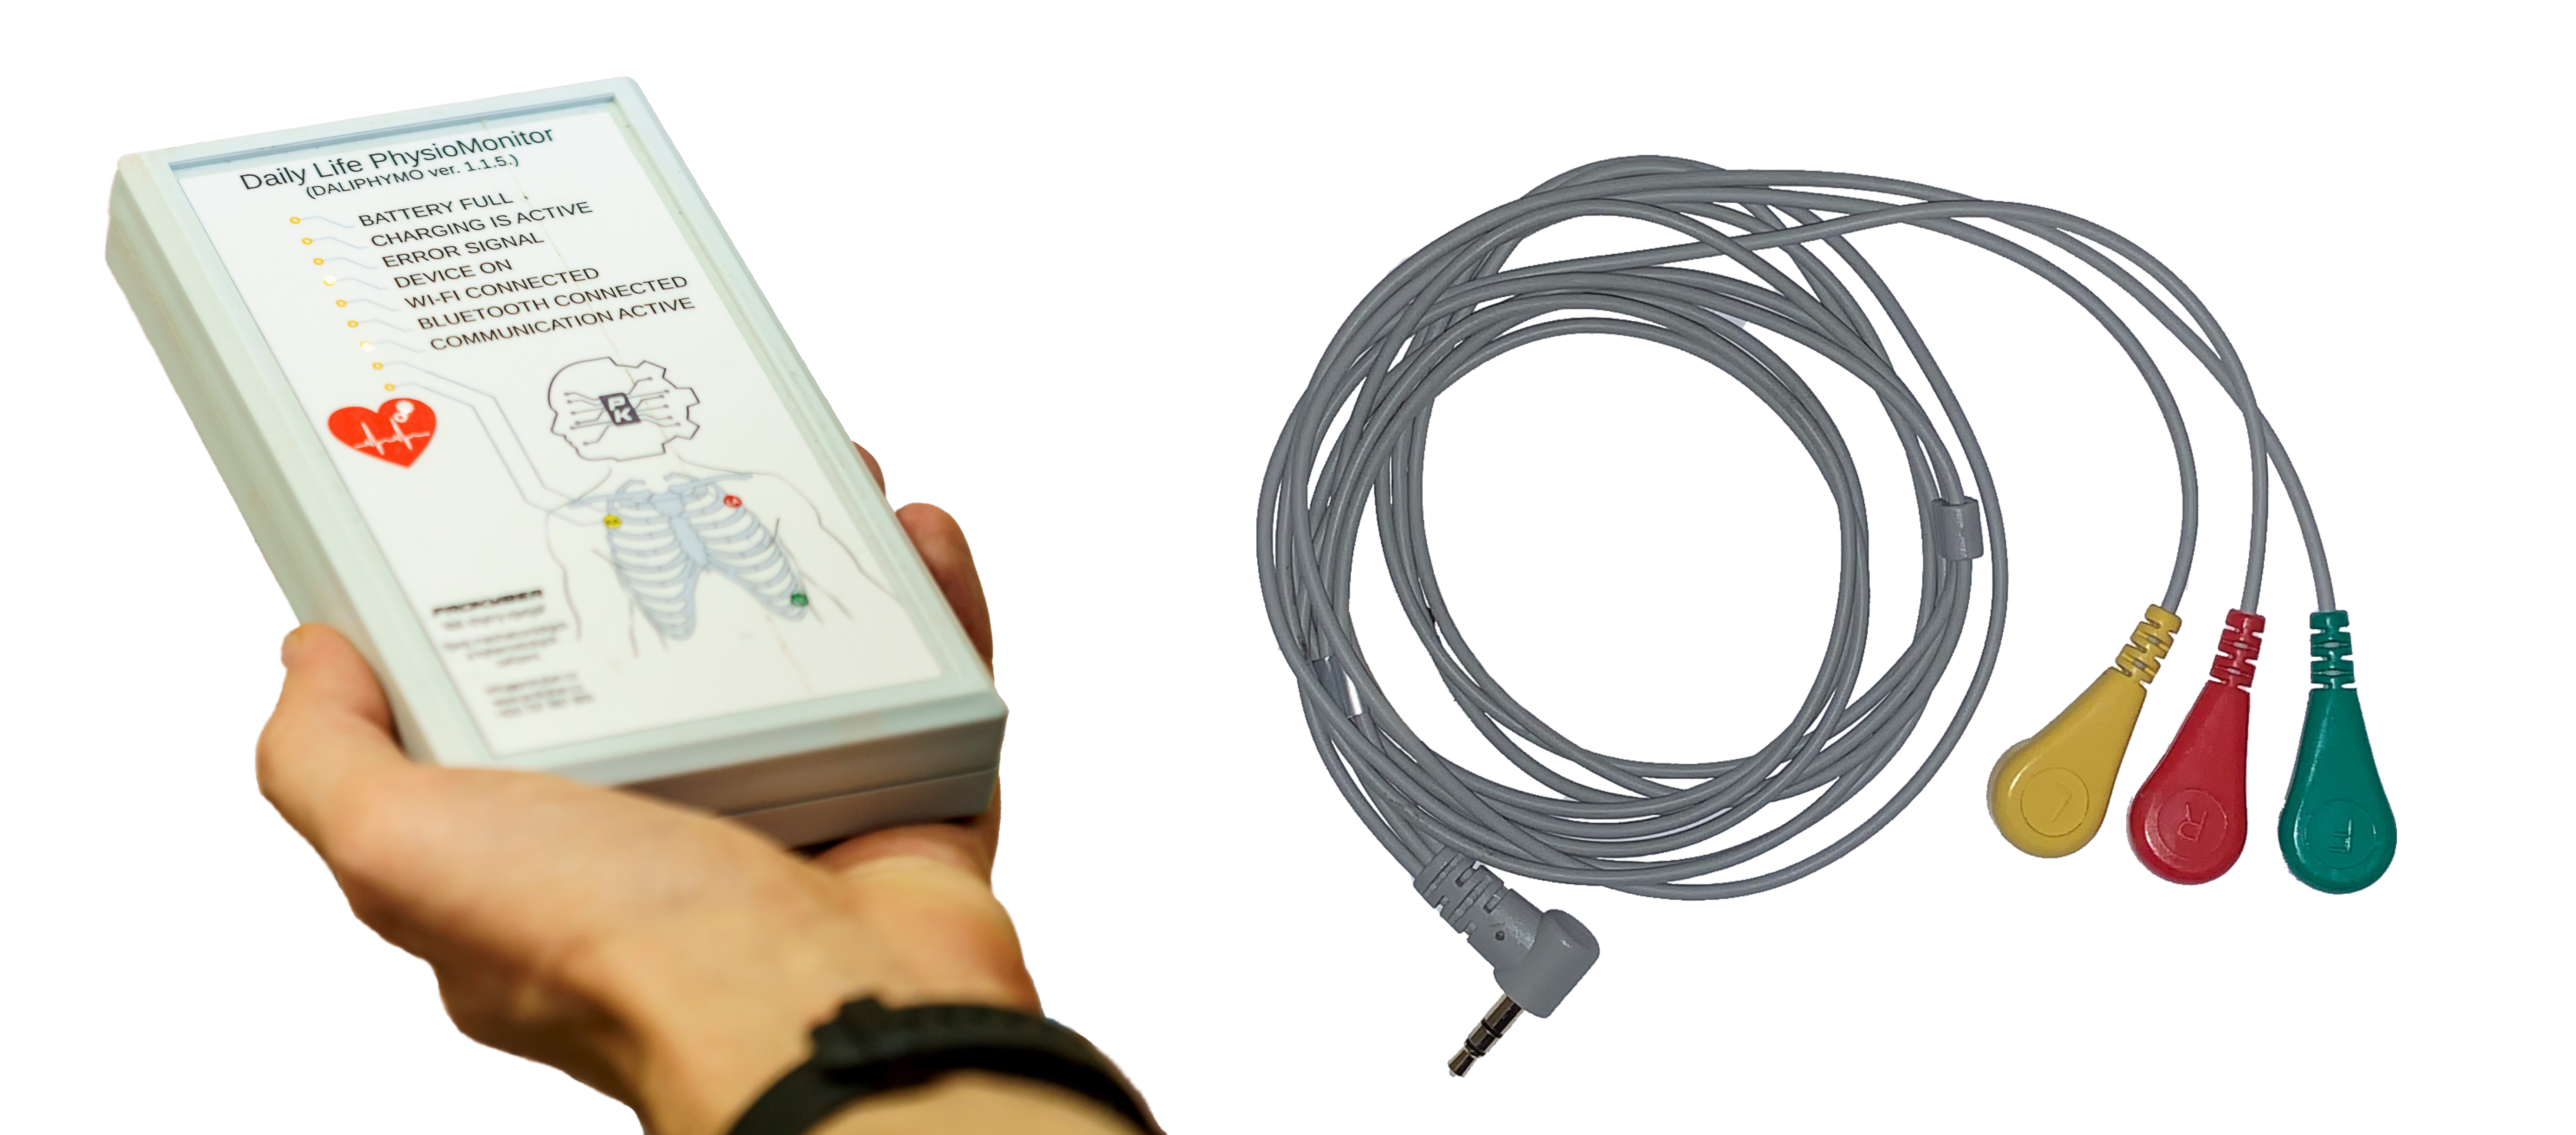
\includegraphics[width=0.9\textwidth]{../assets/device/holter1}
        \caption{Měřící zařízení s příslušenstvím}
        \label{fig:device}
    \end{center}
\end{figure}

Holterův monitor musí být při připojování k bezdrátové sítí v bezprostřední
blízkosti chytrého zařízení, kterým bude konfigurován. Postup pro připojení
měřícího zařízení k WLAN sítí je následující:

\begin{enumerate}
    \item Připojení chytrého mobilního zařízení, které bude sloužit ke
          konfiguraci Holterova monitoru, k požadované WLAN sítí na které bude
          probíhat komunikace.
    \item Přepnutí měřícího zařízení do režimu konfigurace stiskem tlačítka
          \textbf{Config}, které se nachází na horní ploše okraje.
    \item Spuštění aplikace \textit{ESPTouch: SmartConfig}.
    \item Ověření správně vybrané WLAN sítě pomocí identifikátoru \textbf{SSID}
          v horní části úvodní obrazovky aplikace (Obr. \ref{fig:app_screen1}).
    \item Vyplnění hesla v kolonce \textbf{Password} náležícího zvolené WLAN
          sítí. Ostatní parametry jsou ponechány ve výchozím stavu.
    \item Stisk tlačítka \textbf{Confirm} v dolní části aplikace pro zahájení
          konfigurace a připojení Holteru k vybrané sítí.
\end{enumerate}

Pokud se měřící zařízení připojilo úspěšně k vybrané WLAN sítí, objeví se
notifikace jako na Obr. \ref{fig:app_screen2} a zároveň je navázané spojení
indikováno rozsvícenou LED kontrolkou na předním panelu Holteru u položky
\textbf{WI-FI CONNECTED}. Při nezdařeném pokusu připojení je nutné opakovat
kroky od bodu 2 nebo případně zkontrolovat stav baterie Holteru.

\begin{figure}[h]
    \centering
    \begin{subfigure}[b]{0.45\textwidth}
        \centering
        \textcolor{cyan}{\fboxrule=2pt\fboxsep=0pt\fbox{\includegraphics[width=0.8\linewidth]{../assets/device/app_screen1}}}
        \caption{Úvodní obrazovka aplikace}
        \label{fig:app_screen1}
    \end{subfigure}
    \hfill
    \begin{subfigure}[b]{0.45\textwidth}
        \centering
        \textcolor{cyan}{\fboxrule=2pt\fboxsep=0pt\fbox{\includegraphics[width=0.8\linewidth]{../assets/device/app_screen2}}}
        \caption{Notifikace úspěšného připojení}
        \label{fig:app_screen2}
    \end{subfigure}
    \caption{Konfigurace měřícího zařízení v aplikaci \textit{ESPTouch:
            SmartConfig}}
    \label{fig:esptouch_app}
\end{figure}

\subsubsection{Metodika měření}
\label{section:measurement_methodology}
Metodika měření spočívá v krátkodobém záznamu srdeční aktivity ve dvou odlišných
situacích. Před měřením je na subjekt připojeno měřící zařízení
(\ref{section:measurement_device}) pomocí adhezivních EKG elektrod (Obr.
\ref{fig:device_usage}). Jedná se o bipolární hrudní 3-svodové zapojení elektrod
(\ref{section:electrocardiography}). Měření každého záznamu trvá 10 minut,
přičemž se jedná o dva 5 minutové spojité úseky. Subjekt nesmí být před měřením
vystaven fyzické ani psychické zátěži. Během měření v prvním 5 minutovém úseku
je subjekt po celou dobu v klidu. V druhém 5 minutovém úseku je subjekt vystaven
situaci stimulující kognitivní zátěž v podobě Stroopova testu. Stroopův test je
realizován formou videozáznamu a blíže je popsán v následující kapitole. Postup
měření je detailněji popsán v sekci \ref{section:measurement_process}.

\begin{figure}[h]
    \begin{center}
        \includegraphics[width=0.8\textwidth]{../assets/device/holter2}
        \caption{Měření srdeční aktivity}
        \label{fig:device_usage}
    \end{center}
\end{figure}

\subsubsection{Stroopův test}
\label{section:stroop_test}
Stroopův test se řadí mezi psychologické testy osobnosti a byl primárně navržený
pro testování percepční zátěže. Postupem času se možnosti jeho využití
rozšiřovaly \cite{Svoboda1999}. Dnes je Stroopův test jeden z nejběžnějších
neuropsychologických testů používaný k hodnocení  a stimulaci kognitivní zátěže
\cite{Scarpina2017}.

\begin{figure}[h]
    \begin{center}
        \includegraphics[width=1\textwidth]{../assets/figures/stroop}
        \caption{Příklad Stroopova testu \cite{stroopWiki}}
        \label{fig:stroop}
    \end{center}
\end{figure}

Princip testu spočívá ve třech po sobě následujících krocích. Prvním krokem je
přečtení řady slov, která jsou napsaná černou barvou a označují několik barev
(nejčastěji červená, žlutá, zelená a modrá). Dalším krokem je pojmenování každé
jednotlivé barvy v další řadě tvořené barevnými obdélníky. Posledním krokem je
přečtení řady slov, která jsou napsaná barevně ale význam slova této barvě
neodpovídá \cite{Svoboda1999}. Na Obr. \ref{fig:stroop} lze vidět příklad testu.

\subsubsection{Postup měření}
\label{section:measurement_process}
Postup záznamu srdeční aktivity u jednotlivých probandů sestává z
následujících kroků:

\begin{enumerate}
    \item Konfigurace měřícího zařízení podle postupu v sekci
          \ref{section:measurement_device}.
    \item Nalepení elektrod na měřeného probanda podle Obr.
          \ref{fig:device_usage} a připojení příslušných EKG kabelů k elektrodám.
    \item Zapnutí aplikace \textit{BBPM}. Počítač na kterém běží aplikace musí
          být připojený ke stejné sítí jako měřící zařízení.
    \item Nastavení aplikace stiskem tlačítka \textbf{Settings} a vyplněním IP
          adresy a portu měřícího zařízení do kolonek \textbf{Host} a \textbf{Port} v
          kartě \textbf{General}.
    \item Ověření validity spojení stiskem tlačítka \textbf{Test connection}.
    \item Připojení aplikace k měřícímu zařízení stiskem tlačítka
          \textbf{Apply} a následně \textbf{Ok}.
    \item Zahájení záznamu srdeční aktivity stiskem tlačítka \textbf{Record} a
          vybrání cílové destinace, kde bude soubor po ukončení záznamu uložen.
    \item Ukončení záznamu po 10 minutách opětovným stiskem tlačítka \textbf{Record}.
\end{enumerate}

\subsection{Studie}
\label{section:study}
\subsubsection{Kontrolní skupina probandů}
\label{section:probands}
Za účelem otestovaní navrženého řešení v rámci této bakalářské práce (viz
kapitola 3) byla naměřena a zaznamenána srdeční aktivita podle postupu
\ref{section:measurement_process} u kontrolní skupiny 5 probandů ve věkovém
rozmezí 21--23 let bez diagnostikovaných kardiovaskulárních onemocnění.

\subsubsection{Sledované statistické veličiny}
\label{section:selected_stats_vals}
Výstupem aplikace použité k záznamu srdeční aktivity jsou soubory formátu CSV,
kde každý řádek reprezentuje naměřenou elektrickou amplitudu v daný časový
okamžik. Díky znalosti vzorkovací frekvence zařízení lze snadno ke každému
záznamu vypočítat časový vektor a pracovat tak v časové oblasti.

V závislosti na studii byly vybrány následující sledované statistické parametry
Poincarého grafu s vyžitím metody konstrukce elipsy (viz kapitola
\ref{section:hrv_methods}):

\begin{itemize}
    \item \textbf{SD1}~\textit{(Standard Deviation)} --- směrodatná odchylka R-R
          intervalů hlavní osy elipsy,
    \item \textbf{SD2}~\textit{(Standard Deviation)} --- směrodatná odchylka R-R
          intervalů vedlejší osy elipsy,
    \item \textbf{SD1/SD2}~\textit{(Standard Deviation ratio)} --- poměr směrodatných odchylek SD1 a SD2.
\end{itemize}

\subsection{Offline zpracování EKG záznamu}
\label{section:offline_processing}
Zpracování EKG záznamů se orientuje podle diagramu na Obr.
\ref{fig:diagram_offline_processing} níže a je realizováno v prostředí programu
MathWorks MATLAB 2021a. Jednotlivé částí zpracování jsou rozebrány v
následujících kapitolách.

\begin{figure}[H]
    \centering
    \begin{tikzpicture}[node distance=2.5cm, thick, scale=0.8, every node/.style={scale=0.8}]
        \node (start) [startstop, text width=2cm] {EKG záznam};
        \node (pro1) [process, right of=start, xshift=1.5cm] {Předzpracování};
        \node (pro2) [process, right of=pro1, xshift=1.5cm, text width=3cm] {Detekce komponentů};
        \node (pro3) [process, right of=pro2, xshift=1.5cm, text width=3cm] {Zpracování komponentů};
        \node (stop) [startstop, right of=pro3, xshift=1.5cm, text width=3cm] {Hodnocení záznamu};

        \draw [arrow] (start) -- (pro1);
        \draw [arrow] (pro1) -- (pro2);
        \draw [arrow] (pro2) -- (pro3);
        \draw [arrow] (pro3) -- (stop);
    \end{tikzpicture}
    \caption{Diagram offline zpracování EKG záznamu}
    \label{fig:diagram_offline_processing}
\end{figure}

\subsubsection{Předzpracování signálu}
\label{section:preprocessing}
První částí, která je nezbytná pro jakoukoliv další práci s biosignálem, je jeho
filtrace. Před navržením samotného filtru byl proveden rozbor EKG záznamu pomocí
FFT. EKG signál byl tak převeden z časové domény do frekvenční funkcí
\texttt{fft(X)} \cite{matlabFFT}. Z teorie je známo v jakých frekvencích se
vyskytuje užitečný EKG signál nebo jeho komponenty a v jakých nežádoucí vlivy
(viz kapitola \ref{section:ecg_processing_theory}). Tyto znalosti byly při
návrhu filtru a posuzování spektra EKG signálu využity. Pro zlepšení představy o
potenciálních artefaktech a užitečných frekvencích byla provedena FFT analýza i
na několika samotných PQRST segmentech. Na Obr. \ref{fig:spectral_analysis} lze
vidět FFT analýzu EKG signálu a jednoho PQRST segmentu. Z examinace pouhé
vizuální stránky signálu plyne několik východisek pro tvorbu filtru. Jsou zde
pohybové artefakty společně s kolísáním nulové izolinie. Ve frekvenčním spektru
a v částech signálu se dále objevuje nepatrný širokopásmový šum, způsobený
myopotenciály. Ve frekvenčním spektru lze vidět tyto nežádoucí složky přibližně
mezi frekvencemi od 0 do 5--10~\si\Hz.

\begin{figure}[h]
    \begin{center}
        \includegraphics[width=1\textwidth]{../assets/figures/spectral_analysis}
        \caption{FFT analýza EKG signálu a QRS komplexu}
        \label{fig:spectral_analysis}
    \end{center}
\end{figure}

Na základě FFT analýzy byl pro potlačení nežádoucích prvků zvolen digitální
filtr FIR typu pásmová propust s propustnými frekvencemi v rozmezí
7.5--35~\si\Hz. Filtr byl navržen metodou Kaiserova okna \cite{Chavan2006},
které je definované jako \cite{Oppenheim1999}:

\begin{equation}
    \label{eq:kaiser1}
    w[n] =
    \begin{cases}
        \frac{I_0[\beta(1-[(n-\alpha/\alpha]^2)^{1/2}]}{I_0(\beta)}, & 0 \leq n \leq M, \\
        0,                                                           & \text{jinak}
    \end{cases}
\end{equation}

kde $M$ je počet vzorků, $\alpha=M/2$ a $I_0(\cdot)$ reprezentuje 0. řád
modifikované Besselovy funkce prvního druhu \cite{BesselFcn}. Jelikož je potřeba
dosáhnout specifického útlumu $A$ (viz kapitola
\ref{section:ecg_processing_theory}), definoval Kaiser parametr $\beta$
následovně \cite{Oppenheim1999}:

\begin{equation}
    \beta =
    \begin{cases}
        0.1102(A-8.7),                    & A > 50            \\
        0.5842(A-21)^0.4 + 0.07886(A-21), & 21 \leq A \leq 50 \\
        0.0,                              & A < 21.
    \end{cases}
\end{equation}

Filtr byl realizován funkcí \texttt{bandpass(x,fpass,fs)} \cite{matlabBANDPASS}.
Druhou části předzpracování tvoří filtrace zvýrazňující QRS komplexy, konkrétně
R vlny. Použitá metoda pro zvýraznění vychází z vlastností derivace a vyšších
amplitud R vln. Filtrovaný signál je nejdříve diferencován použitím pěti-bodové
diference prvního řádu dle následujícího vztahu \cite{Wang2017}:

\begin{equation}
    \label{eq:differentiation}
    d[n] = \frac{1}{8}(2f[n] + f[n-1] - f[n-3] - 2f[n-4])
\end{equation}

kde $n \geq 5$, $d[n]$ reprezentuje vzorek diferencovaného signálu a $f[n]$
hodnotu původního vzorku. Diferenciace zároveň potlačuje vlivy P a T vln.
Výstupem diferenciace je bipolární signál, který je umocněn. QRS regiony jsou
následně jednotlivě sloučeny a zvýrazněny využitím zpětné kumulace
\cite{Wang2017}:
\begin{equation}
    \label{eq:backward_cumulation}
    Bc(n) = \sum_{i=n}^{n+Ww-1} |d(i)|
\end{equation}
s pevným oknem $(Ww)$ v rozsahu nejdelšího normálního trvání jednoho QRS
komplexu (0,12 s) \cite{Wang2017}. Ke kumulaci je využívána funkce
\texttt{cumsum(A)} \cite{matlabCUMSUM}.

\begin{figure}[h]
    \begin{center}
        \includegraphics[width=1\textwidth]{../assets/figures/preprocessing_steps}
        \caption{Jednotlivé kroky předzpracování EKG signálu}
        \label{fig:preprocessing_steps}
    \end{center}
\end{figure}

Poslední krok předzpracování je vyhlazení vzniklých vrcholů konvolucí, funkcí
\texttt{conv(u,v)} \cite{matlabCONV}. Konvoluční kernel je tvořen podílem
jednotkového vektoru o délce 60 vzorků a délkou vektoru. Délka 60 vzorků je
stejně jako u zpětné kumulace doba trvání QRS komplexu, převedena z času na
počet vzorků pomocí vzorkovací frekvence (500~\si\Hz). Vizuálně lze vidět
jednotlivé kroky předzpracování signálu na Obr. \ref{fig:preprocessing_steps}.

\subsubsection{Detekce komponentů}
\label{section:components_detection}
Vzhledem k charakteru analýzy EKG záznamů v rámci této práce jsou předmětem
detekce pozitivní kmity signálu neboli R vlny. Za účelem detekce R vln byl
implementován a modifikován algoritmus podle \cite{Nabian2018}, inspirovaný
Pan-Tompkinsovou metodou QRS detekce \cite{Pan1985} (viz kapitola
\ref{section:components_detection_theory}). Algoritmus vychází z následujících
kroků \cite{Nabian2018}:

\begin{enumerate}
    \item Iterativní hledání globálních maximálních amplitud s použitím
          plovoucího okna $W$ o délce 400~\si\ms~(0,4~\si\s):
          \begin{gather}
              R_i = max(W_i^{L,R}) \nonumber \\
              W_i^{L,R} = \{x_{i-L},...,x_i,...,x_{i+R}\} \nonumber \\
              L = R = \frac{0.4}{2} Fs
          \end{gather}
          kde $Fs$ je vzorkovací frekvence, $R_i$ potenciální R vlna, $x_i$
          střed okna a $L$ spolu s $R$ posun od středu plovoucího okna. Nalezená
          maxima nacházející se uprostřed plovoucího okna jsou označeny jako
          potenciální R vlny.
    \item Eliminace všech R vln nižších než než prahová hodnota $Th_{Amp}$, která je v
          každé iteraci rovna 75 \% z průměru amplitůd posledních 8 detekovaných
          R vln. Iniciálně je prahová hodnota $Th_{Amp}$ nastavena jako:
          \begin{gather}
              N = 2~Fs \nonumber \\
              Th_{Amp} = \frac{1}{3} max(\{x_1,x_2,x_3,...,x_N\})
          \end{gather}
    \item Výpočet R-R intervalů ($RR_i$) diferencí detekovaných R vln ($R_i$):
          \begin{equation}
              RR_i = R_{i+1} - R_i
          \end{equation}
          a následná iterativní kontrola vypočítaných R-R intervalů. Intervaly
          delší než prahová hodnota $Th_{RR}$ indikují chybějící R vlnu, která je
          doplněna jako maximální amplituda mezi sousedními R vlny v délce
          plovoucího okna. Prahová hodnota $Th_{RR}$ je počátečně nastavena jako:
          \begin{equation}
              Th_{RR} = 1.66~RR_1
          \end{equation}
\end{enumerate}

Délka plovoucího okna se řídí fyziologickým limitem hodnoty srdečního rytmu v
případech jako jsou například supraventrikulární tachykardie (SVT) nebo flutter
síní, kde dosahuje srdeční frekvence přibližně 300 úderů za minutu (5 úderů za
sekundu) \cite{Haberl2012,Goldberger2017}. Dva sousední QRS komplexy se tedy
nemůžou vyskytnout blíže než 200~\si\ms. Další zbylé komponenty (P, Q, S, T) lze
detekovat využitím fyziologických časových hodnot těchto komponentů a R vln jako
referenčních bodů k nalezení jejich pozic \cite{Nabian2018}. Na Obr.
\ref{fig:detection} lze vidět zeleně vyznačený adaptivní práh, který se mění podle
2. kroku výše a doplněnou R vlnu, která nebyla detekovaná v 1. kroku ale až ve
3. a následně přidána.

\begin{figure}[h]
    \begin{center}
        \includegraphics[width=1\textwidth]{../assets/figures/detection}
        \caption{Detekce R vln}
        \label{fig:detection}
    \end{center}
\end{figure}

Aby bylo možné detekované vlny vizualizovat na původním signálu jako je tomu na
Obr. \ref{fig:detection}, byla zavedena metoda relokalizace, která upraví pozice
detekovaných R vln tak, aby souhlasily v původním EKG záznamu. Postup metody se
řídí diagramem na Obr. \ref{fig:fixpeaks}, kde $X$ reprezentuje pole hodnot EKG
signálu.

\begin{figure}[h]
    \begin{center}
        \includegraphics[width=0.8\textwidth]{../assets/figures/fixpeaks}
        \caption{Relokalizace nalezených R vln}
        \label{fig:fixpeaks}
    \end{center}
\end{figure}

\subsubsection{Zpracování komponentů}
\label{section:components_processing}


\subsubsection{Analýza zpracovaného záznamu}
\label{section:analyze}

\subsection{Online zpracování EKG záznamu}
\label{section:online_processing}

\subsection{Statistické metody}
\label{section:statistical_methods}